\documentclass[10pt,a4paper]{article}
\usepackage[margin=2.2cm]{geometry}
\usepackage{fontspec}
\usepackage{kotex}
\setmainfont{Apple SD Gothic Neo}
\setsansfont{Apple SD Gothic Neo}
\usepackage{amsmath,amssymb}
\usepackage{graphicx}
\usepackage{booktabs}
\usepackage{caption}
\usepackage[dvipsnames]{xcolor}
\usepackage[colorlinks=true,linkcolor=MidnightBlue,citecolor=MidnightBlue,
            urlcolor=MidnightBlue]{hyperref}
\usepackage{titlesec}
\titleformat{\section}{\large\bfseries}{\thesection}{0.6em}{}
\titleformat{\subsection}{\normalsize\bfseries}{\thesubsection}{0.5em}{}
\captionsetup{font=small,labelfont=bf}
\setlength{\parskip}{0.35em}
\setlength{\parindent}{0pt}

\usepackage{mdframed}
\newmdenv[linewidth=0.4pt,linecolor=gray!60,backgroundcolor=gray!5,
          innertopmargin=6pt,innerbottommargin=6pt,skipabove=8pt,skipbelow=8pt]{claimbox}
\newcommand{\claim}[2]{\begin{claimbox}\textbf{주장.} #1\par\smallskip
  \textcolor{gray!70}{\textbf{반증 조건.} #2}\end{claimbox}}

\title{\bfseries 4{,}132개의 봉투\\[2pt]
\large 처음으로 미래를 향해 적었고, 그러다 내 반박이 반쪽이었음을 알았다}
\author{월드모델 실험실 · 노트 694}
\date{2026-08-06}
\begin{document}\maketitle

\section{한 줄}

아직 각색 안 된 만화 \textbf{4{,}132건}에 선별 확률을 봉인했다 --- 이 실험실
\textbf{첫 전향 기록}이다. 그 김에 ``애니 흥행은 제작사가 지배한다''는 외부
비평을 명시적으로 쟀는데 \textbf{제작사가 아무것도 더하지 않았다}(B$-$A $=-0.002$,
위약과 차 $0.0005$). 그리고 \textbf{내 앞선 반박이 방법상 반쪽이었음}을 알았다 ---
$154$모수와 $2$모수를 표본 안에서 견줬다.

\section{봉투를 봉하는 규율 넷}

지금까지 모든 숫자가 T 유보 백테스트고 전향 기록이 \textbf{0건}이었다. 노트 693 이
그것을 능력 카드의 \emph{금지 꼴}로 박았다(``지금까지 ○○\% 적중''을 말할 수 없다).
백테스트만 들고 협력 자리에 가면 첫 질문에서 걸린다.

봉인은 \textbf{되돌릴 수 없어야} 값이 있다. 그래서 규율을 넷 뒀다.

\begin{center}
\begin{tabular}{ll}
\toprule
① 모형 지문을 같이 적는다 & 특징 7 · 버린 특징 6 · 코드 \texttt{sha256 372497a5} · 자료 스냅샷 \\
② 오늘을 하드 컷오프로 & 봉인 시각과 스냅샷 크기(만화 7{,}982 · 각색 짝 564) \\
③ 파일을 다시 쓰지 않는다 & 같은 날 두 번 부르면 \texttt{FileExistsError} --- 시험했다 \\
\textbf{④ 채점 규칙을 봉인 때 적는다} & \textbf{뒤에 정하면 그것이 체리피킹이다} \\
\bottomrule
\end{tabular}
\end{center}

④가 핵심이다. 봉인 파일 \emph{안}에 양성 정의 · 판정 표본(상위 100) · 창(24개월) ·
판정선(3건 이하면 실패) · \textbf{대조(하위 100건도 센다)} 를 넣었다. 다음 세션이
그것을 못 바꾼다.

\claim{\textbf{대조 없는 전향 채점은 기저율 변화와 구분되지 않는다.} 상위 100건의
양성 수만 보면 그 해에 각색이 늘었을 뿐인 것을 성공으로 읽는다. 그래서 같은 창의
\textbf{하위 100건}을 같이 센다 --- 둘이 같으면 순위가 시간에 안 옮겨간 것이다.}
{하위 100건은 확률 $5\times10^{-5}$ 대역이라 24개월 안 양성이 0일 수 있다. 그러면
대조가 정보를 안 주고, 중간 구간(예: 순위 1{,}000--1{,}100)을 대조로 바꿔야 한다.}

배선도 검사했다 --- 봉인 행수 $4{,}132$ = 유보 $4{,}263$ $-$ 양성 $131$ 로 일치한다.

\subsection*{그리고 예측을 봉인 안에 적었다}

상위 100건 중 24개월 안 \textbf{8--20건}. \textbf{한계도 같이 적었다}: 캘리브레이션
$0.2713 \to 0.2290$ 은 유보 \emph{전체}(이미 각색된 것 포함)에서 나온 값이고, 봉인
대상은 ``아직 각색 안 된'' 조건부라 \textbf{잔여 비율}이므로 그보다 낮아야 한다.

\section{제작사를 명시적으로 넣었더니 아무 일도 없었다}

\begin{figure}[t]\centering
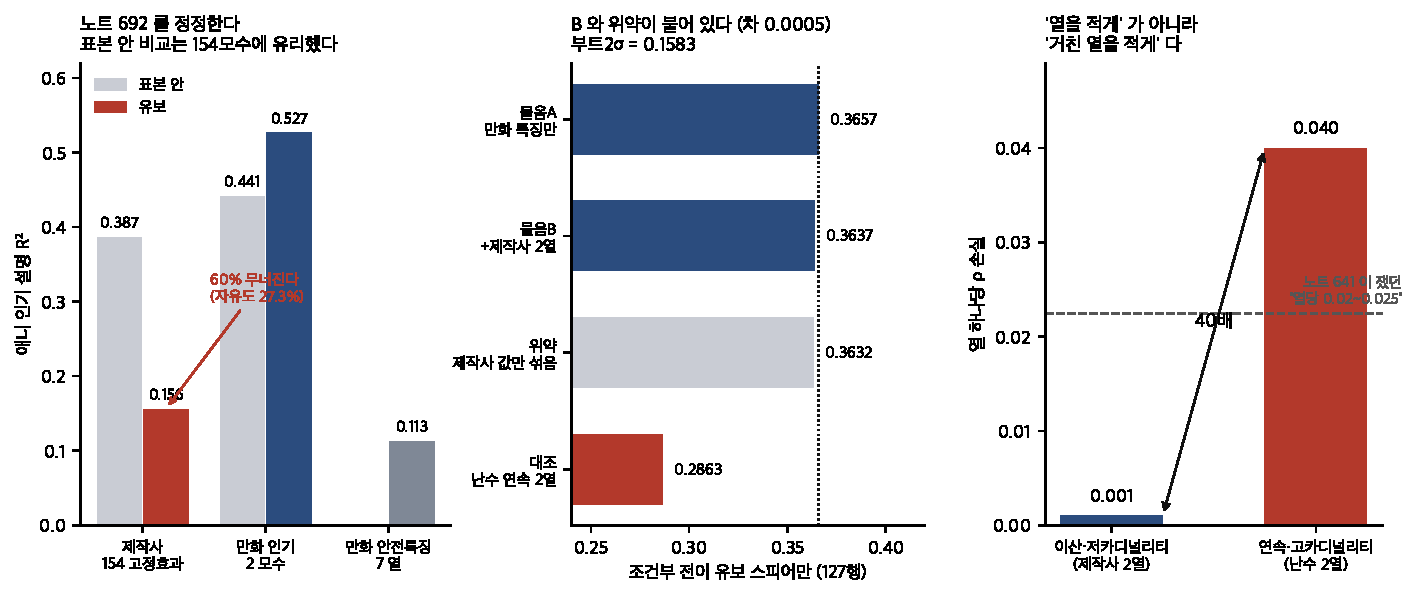
\includegraphics[width=0.99\textwidth]{figs/sealed.pdf}
\caption{왼쪽: 표본 안과 유보. \textbf{제작사는 60\% 무너지고 만화 인기는 오른다.}
가운데: 제작사 2열을 얹은 팔이 \textbf{자기 위약과 붙어 있다.} 오른쪽: 같은 2열인데
비용이 40배 다르다.}
\end{figure}

564 각색 짝(학습 437 · 유보 127 · 제작사 이름 564/564)에서 네 팔을 돌렸다. 제작사는
\textbf{라벨 없이} 인코딩했다 --- 학습 행의 제작 편수 로그와 학습 상위 10곳 지시자
두 열뿐이다(라벨로 체급을 만들면 그것이 누출이다 · 노트 645).

\begin{center}
\begin{tabular}{lrl}
\toprule
팔 & 유보 스피어만 & \\
\midrule
물음A --- 만화 특징만(기획 시점) & $0.3657$ & \\
물음B --- $+$ 제작사 2열 & $0.3637$ & $-0.002$ \\
\textbf{위약} --- 제작사 \emph{값만} 섞음 & $\mathbf{0.3632}$ & \textbf{B 와 차 $0.0005$} \\
대조 --- 난수 연속 2열 & $0.2863$ & $-0.0794$ \\
\bottomrule
\end{tabular}
\end{center}

부트스트랩 $2\sigma$ 가 $0.1583$ 이므로 B$-$A 는 문턱 근처도 아니다. 그리고 노트 335
의 규율이 그대로 발동한다 --- \textbf{위약이 진짜보다 나쁘지 않으면 신호가 아니다.}

\claim{\textbf{제작사는 만화 특징에 이미 담겨 있다.} 기제도 나왔다 --- 제작사의
\emph{유보} R$^2$ 가 $0.1559$ 이고 만화 안전특징의 유보 R$^2$ 가 $0.1127$ 로 가깝다.
\textbf{둘이 같은 것을 잰다}: 큰 제작사가 인기 갈래를 맡는다. 그것이 ``제작사 배정은
외생이 아니다''(역인과)의 자료 쪽 지문이다.}
{제작사를 2열로 뭉갰다. 유보 127행에 154 원핫은 불가능하므로 \textbf{개별 제작사
효과는 못 봤다}. 짝이 수천 건으로 자라면 다시 재야 하고, 그때 이 주장은 ``체급
두 열로는'' 으로 좁혀진다.}

\subsection*{내가 틀린 자리 --- 앞선 반박이 반쪽이었다}

노트 692 는 \emph{``제작사 R$^2$ $0.3865$ $<$ 만화 라벨 $0.4412$ 이므로 비평이
틀렸다''}고 적었다. \textbf{둘 다 표본 안 값이었다.} 유보로 다시 재니:

\begin{center}
\begin{tabular}{lrr}
\toprule
 & 표본 안 & 유보 \\
\midrule
제작사 154 고정효과 & $0.3865$ & $\mathbf{+0.1559}$ \\
만화 인기 2 모수 & $0.4412$ & $\mathbf{+0.5266}$ \\
\bottomrule
\end{tabular}
\end{center}

제작사는 자유도 $154/564 = 27.3\%$ 때문에 \textbf{60\% 무너지고}, 만화 인기는 모수가
둘뿐이라 \textbf{오히려 오른다}.

\claim{\textbf{결론은 같고 근거는 더 강해졌지만 방법은 내가 틀렸다.} 유보 격차는
$3.4$배($0.1559$ 대 $0.5266$)로 표본 안보다 훨씬 크다. 그러나 \textbf{$154$모수와
$2$모수를 표본 안에서 견주는 것은 제작사에 유리한 비교}였고, 진짜 논거는 ``유리한
비교에서도 만화가 이겼다''가 아니라 \textbf{``공정한 자(유보)에서 3.4배''} 다.}
{모수 수를 벌하는 자(조정 R$^2$ · AIC)로 표본 안에서 견주면 유보 없이도 같은 결론이
날 수 있다. 그러면 이 주장은 ``표본 안 R$^2$ 로는'' 으로 좁혀진다.}

\section{곁가지가 제일 클지도 모른다 --- 차원 비용은 거칠기에 달렸다}

같은 \textbf{2열}인데 비용이 다르다. 난수 연속 2열은 $-0.0794$(열당 $0.040$)이고
이산 제작사 2열은 $-0.002$(열당 $0.001$)다. \textbf{40배}.

\claim{\textbf{노트 641 의 ``얇은 도메인에서 열 하나당 $\rho$ $0.02$--$0.025$'' 는
고정값이 아니다.} 연속 · 고카디널리티 열은 트리가 과적합할 여지가 커서 비싸고,
저카디널리티 이산 열은 거의 공짜다. 그러므로 규율이 \textbf{``열을 적게''에서
``거친 열을 적게''} 로 바뀐다 --- 이것은 앞으로 후보 축을 고르는 기준을 바꾼다.}
{표본 하나(564행 짝)에서 두 점만 봤다. 판에서 카디널리티 층별로(이진 · 십분위 ·
연속) 쓰레기 열을 넣어 곡선을 만들어야 주장이 선다. \textbf{그것이 T4 의 다음
실험으로 등록됐다.} 곡선이 평평하면 이 관측은 짝 도메인의 특성이다.}

\section{그래서 지금 무엇을 말할 수 있나}

\begin{itemize}
\item \textbf{전향 기록이 0건에서 1건(4{,}132 예보)이 됐다.} 다만 채점은 24개월
      뒤다 --- 당일에 채점을 부르면 코드가 \emph{``아직 아무것도 안 말한다''}를 낸다.
\item 외부 비평의 세 지적 중 \textbf{둘이 자료에서 죽었다} --- 대조군은 있고
      (비각색 만화 7{,}421건) 제작사는 안 더한다. 남은 하나(생존 편향 $27$배)는
      \textbf{맞고, 그래서 2단 모형이 있다.}
\item \textbf{내 반박의 방법을 정정했다.} 장부에 ``노트 692 의 R$^2$ 비교를 그대로
      인용하지 않는다''를 결정 규칙으로 달았다.
\end{itemize}

\end{document}
